\documentclass[a4paper,11pt]{article}
\input{/home/tof/Documents/Cozy/latex-include/preambule_doc.tex}
\input{/home/tof/Documents/Cozy/latex-include/preambule_commun.tex}
\newcommand{\showprof}{show them}  % comment this line if you don't want to see todo environment
\setlength{\fboxrule}{0.8pt}
\fancyhead[L]{\fbox{\Large{\textbf{ArchMat 01}}}}
\fancyhead[C]{\textbf{Modèle de von Neumann}}
\newdate{madate}{10}{09}{2020}
%\fancyhead[R]{\displaydate{madate}} %\today
\fancyhead[R]{Première - NSI}
\fancyfoot[L]{\vspace{1mm}Christophe Viroulaud}
\AtEndDocument{\label{lastpage}}
\fancyfoot[C]{\textbf{Page \thepage/\pageref{lastpage}}}
\fancyfoot[R]{\includegraphics[width=2cm,align=t]{/home/tof/Documents/Cozy/latex-include/cc.png}}

\begin{document}
Ordinateur de bureau, ordinateur portable, smartphone, tablette, montre connectée, voiture autonome\dots toutes ces machines ont envahi notre quotidien.
\begin{center}
    \framebox{Peut-on décrire une architecture commune à toutes ces machines?}
\end{center}
\section{Première approche}
Dans un ordinateur on retrouve:
\begin{itemize}
    \item un microprocesseur ou CPU (Control Processing Unit),
    \item la mémoire; il en existe plusieurs types:
    \begin{center}
        \centering
        \includegraphics[width=8cm]{ressources/memoires.jpg}
        \captionof{figure}{Plus la mémoire est rapide plus elle est proche du CPU.}
        \end{center}
    \item les entrées / sorties.
\end{itemize}
\section{Le modèle de von Neumann}
\begin{center}
    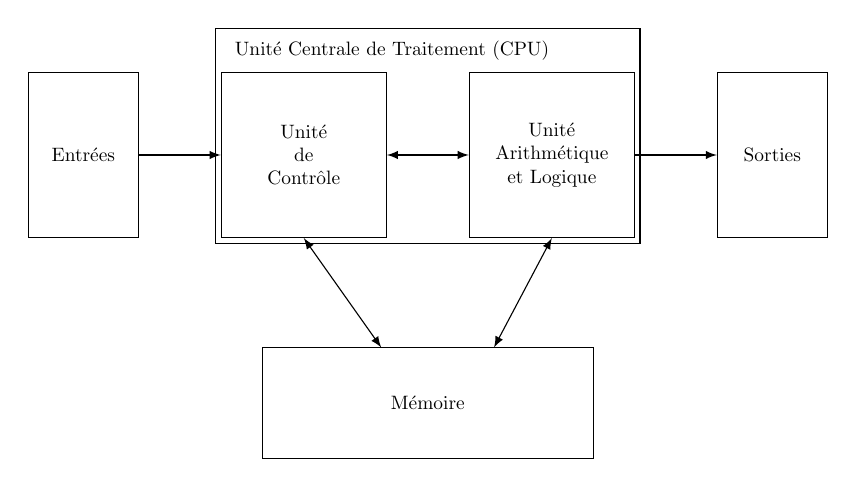
\begin{tikzpicture}[every text node part/.style={align=center},scale=0.7, transform shape]
        \draw (-0.1,-0.1)--(7.6,-0.1)--(7.6,3.8)--(-0.1,3.8)--cycle;
        \node at (3.1,3.4) {Unité Centrale de Traitement (CPU)};
        \node[draw,minimum width=3cm,minimum height=3cm] (uc) at (1.5,1.5){Unité \\ de \\ Contrôle};
        \node[draw,minimum width=3cm,minimum height=3cm] (ual) at (6,1.5){Unité \\ Arithmétique \\ et Logique};

        \node[draw,minimum width=6cm,minimum height=2cm] (mem) at (3.75,-3){Mémoire};
        \node[draw,minimum width=2cm,minimum height=3cm] (i) at (-2.5,1.5){Entrées};
        \node[draw,minimum width=2cm,minimum height=3cm] (o) at (10,1.5){Sorties};
        \draw[<->,>=latex] (ual.south) -- (mem.40);
        \draw[<->,>=latex] (uc.east) -- (ual.west);
        \draw[->,>=latex] (i.east) -- (uc.west);
        \draw[<->,>=latex] (uc.south) -- (mem.130);
        \draw[->,>=latex] (ual.east) -- (o.west);

    \end{tikzpicture}
\end{center}
Ce principe présenté en 1945 par John von Neumann définit encore aujourd'hui le modèles des ordinateurs. Les idées principales sont de: 
\begin{itemize}
    \item considérer un programme comme une donnée. Il sera stocké dans la mémoire
    \item séparer l'unité de commande et l'unité arithmétique.
\end{itemize} 
\section{Un modèle hérité}
Les calculateurs précédents l'avènement du concept de von Neumann souffraient d'un défaut majeur: ils ne pouvaient exécuter qu'un seul programme à la fois. Il fallait reconfigurer la machine pour remplir une autre tâche.
\begin{center}
    \centering
    \includegraphics[width=6cm]{ressources/configeniac.jpg}
    \captionof{figure}{Opératrices configurant l'ENIAC}
    \label{IMG}
    \end{center}
\end{document}